\documentclass[a4paper]{article}
\usepackage{amsmath}
\usepackage{amssymb}
\usepackage{braket}%量子力学符号
\usepackage{geometry}
\usepackage{enumerate}
\usepackage{natbib}
\usepackage{float}%稳定图片位置
\usepackage{graphicx,subfig}%画图
\usepackage{caption}
\usepackage[english]{babel}
\usepackage{indentfirst}%缩进
\usepackage{enumerate}%加序号
\usepackage{multirow}%合并行
\usepackage{hyperref}
\hypersetup{hypertex=true, colorlinks=true, linkcolor=black, anchorcolor=black, citecolor=black}
\title{\Large \textbf{VE485 HomeWork 6}\\
\author{\textbf{Pan, Chongdan ID:516370910121}\\
}
}
\begin{document}
\maketitle
\section{LS Problem}
\noindent To $\min_x ||Ax-b||$, it's equal to minimize $f(x)=(Ax-b)^T(Ax-b)$
\\It's gradient is $\bigtriangledown f(x)=2A^T(Ax-b)$
\\When $f(x)=0$, we get the pseudo inverse $\hat{x}=A^T(AA^T)^{-1}b$
\\I set the $A,X,b$ randomly, stopping critera $\epsilon=0.01$
\\For Backtracking search $\alpha=0.2,\beta=0.25$
\\After a lot of test, I get results similar to following table
\begin{table}[H]
    \centering
    \begin{tabular}{|l|l|l|l}
    \cline{1-3}
    \multicolumn{1}{|c|}{Input} & \multicolumn{1}{c|}{Final Error} & \multicolumn{1}{c|}{Iterations} &  \\ \cline{1-3}
    $\hat{x}$       &  31.57    &0      &  \\ \cline{1-3}
    $0.5\hat{x}$    &  31.57    &30     &  \\ \cline{1-3}
    $0.75x$         &  7.892    &28     &  \\ \cline{1-3}
    $0.25x$         &  23.67    &31     &  \\ \cline{1-3}
    Random          &  44.61    &33     &  \\ \cline{1-3}
    $x$+Random      &  30.81    &30     &  \\ \cline{1-3}
    1               &  43.64    &33     &  \\ \cline{1-3}
    0               &  31.57    &31     &  \\ \cline{1-3}
    0.5             &  54.87    &31     &  \\ \cline{1-3}
    \end{tabular}
\end{table}
\section{Analysis}
For $X_{input}=\hat{x}$, I think it may be a saddle point since it has 0 iterations but still have error between $X$. It may also because $A$ is not symmetric. What's more, if $X_{input}=k\hat{x}$, it will lead to same error after some iterations.
\par For $X_{input}=kX$, it's surprising that $kX$'s error is always lower when $X_{input}=\hat{x}$, hence, they can also lead to similar saddle point, but it's closer to the optimal value, hence there are multiple saddle points. When $k\rightarrow1$, the error is smaller because it's saddle point is closer to the original solution.
\par For $X_{input}=X_{random}$, we can find it always achieves the largest error with most iterations, it may because there are too much saddle points away from $X$ and the random X will lead to it. But I also found that when $X_{input}=X_{random}+X$, error will be smaller.
\par For constant matrix, we find it will lead to results similar to $\hat{x}$, this may have relation with sparsity.
\section{With Noise}
\subsection{Model for $Ax=b$}
    If we use the old model for $Ax=b$, we will get similar result when the noise $\sigma^2$ is small, such as $\sigma\in(0,10)$
    \begin{table}[H]
        \centering
        \begin{tabular}{|l|l|l|l}
        \cline{1-3}
        \multicolumn{1}{|c|}{Input} & \multicolumn{1}{c|}{Final Error} & \multicolumn{1}{c|}{Iterations} &  \\ \cline{1-3}
        $\hat{x}$       &  30.52    &0      &  \\ \cline{1-3}
        $0.5\hat{x}$    &  30.52    &29    &  \\ \cline{1-3}
        $0.75x$         &  7.839    &29    &  \\ \cline{1-3}
        $0.25x$         &  22.93    &31    &  \\ \cline{1-3}
        Random          &  43.33    &32    &  \\ \cline{1-3}
        $x$+Random      &  31.26    &31    &  \\ \cline{1-3}
        1               &  43.24    &32    &  \\ \cline{1-3}
        0               &  30.52    &31    &  \\ \cline{1-3}
        0.5             &  34.17    &30    &  \\ \cline{1-3}
        \end{tabular}
        \caption{When $\sigma=10$}
    \end{table}
    However, when $\sigma$ increase bigger, all error will approach the same value.
    \begin{table}[H]
        \centering
        \begin{tabular}{|l|l|l|l}
        \cline{1-3}
        \multicolumn{1}{|c|}{Input} & \multicolumn{1}{c|}{Final Error} & \multicolumn{1}{c|}{Iterations} &  \\ \cline{1-3}
        $\hat{x}$       &  2230     &0      &  \\ \cline{1-3}
        $0.5\hat{x}$    &  2230     &43     &  \\ \cline{1-3}
        $0.75x$         &  2230     &44     &  \\ \cline{1-3}
        $0.25x$         &  2230     &44     &  \\ \cline{1-3}
        Random          &  2230     &44     &  \\ \cline{1-3}
        $x$+Random      &  2230     &44     &  \\ \cline{1-3}
        1               &  2230     &44     &  \\ \cline{1-3}
        0               &  2230     &44     &  \\ \cline{1-3}
        0.5             &  2230     &44     &  \\ \cline{1-3}
        \end{tabular}
        \caption{When $\sigma=100$}
    \end{table}
    \begin{figure}[H]
        \centering
        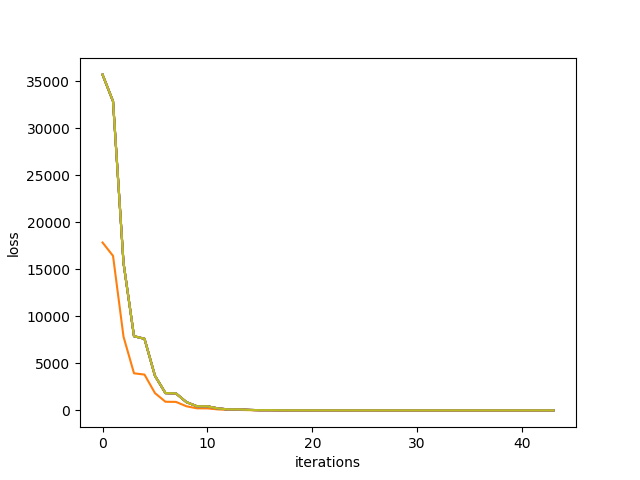
\includegraphics[scale=0.5]{Loss.png}
        \caption{Loss vs. iteration for GD model without considering $\sigma=100$}
    \end{figure}
    The iteration for $\hat{x}$ is still 0, which means it's still at the saddle point. The error will also increase with the increase of $\sigma$. It also takes more iterations to get the optimal value.
\subsection{Model for $Ax+\varepsilon=b$}
    In this case, our objective is to minimize $||Ax+\varepsilon-b||$, hence the gradient $\bigtriangledown f(x)=2A^T(Ax+\varepsilon-b)$, $\hat{x}$ is also $\hat{x}=A^T(AA^T)^{-1}(b-\varepsilon)$ now.
    \par After we change $f(x),\bigtriangledown f(x)$, and $\hat{x}$, we can get same result as $\varepsilon=0$ no matter how large $\varepsilon$
    \begin{figure}[H]
        \centering
        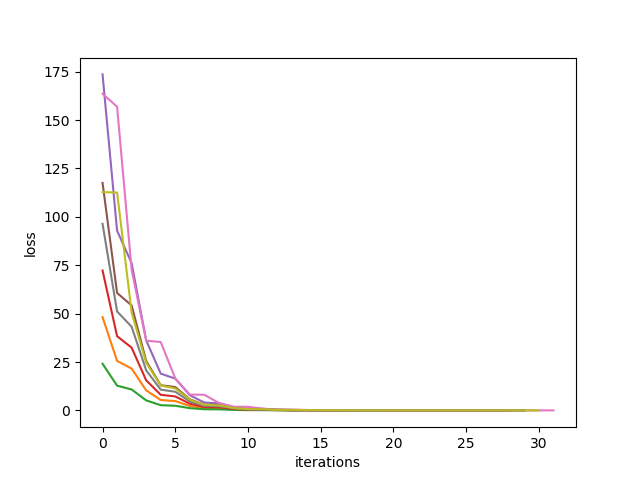
\includegraphics[scale=0.5]{Loss2.png}
        \caption{Loss vs. iteration for GD model considering $\sigma=100$}
    \end{figure}
    \begin{table}[H]
        \centering
        \begin{tabular}{|l|l|l|l}
        \cline{1-3}
        \multicolumn{1}{|c|}{Input} & \multicolumn{1}{c|}{Final Error} & \multicolumn{1}{c|}{Iterations} &  \\ \cline{1-3}
        $\hat{x}$       &  31.77    &0      &  \\ \cline{1-3}
        $0.5\hat{x}$    &  31.77    &29     &  \\ \cline{1-3}
        $0.75x$         &  7.94     &27     &  \\ \cline{1-3}
        $0.25x$         &  23.83    &30     &  \\ \cline{1-3}
        Random          &  45.17    &31     &  \\ \cline{1-3}
        $x$+Random      &  32.37    &30     &  \\ \cline{1-3}
        1               &  43.60    &32     &  \\ \cline{1-3}
        0               &  31.77    &30     &  \\ \cline{1-3}
        0.5             &  34.91    &30     &  \\ \cline{1-3}
        \end{tabular}
        \caption{When $\sigma=100$}
    \end{table}
\section*{Python Code}
\begin{verbatim}
    import numpy as np
    import matplotlib.pyplot as plt
    # loss function
    def loss(A, b, X, delta):
        y = np.dot(A, X) + delta - b # 50*1
        return np.dot(y.T, y)
    
    # GD algorithm
    def GD(A, b, X0, delta):
        e = 1e-2
        a = 0.2
        beta=0.25
        k = 0
        X = X0
        g = 2*np.dot(A.T,np.dot(A,X) + delta - b)
        n = []
        m = []
        while np.linalg.norm(g)>e: # When the gradient is not small enough
            g=2*np.dot(A.T,np.dot(A,X) + delta - b) # Calculate the negative gradient 1000*1
            t=1   
            while 1: # Backtracking
                Xt = X-t*g # 1000*1
                if loss(A, b, Xt, delta) < loss(A, b, X, delta) + a*t*np.dot(g.T, (Xt - X)):
                    break
                t *= beta
            X = Xt
            n.append(k)
            m.append(np.linalg.norm(np.dot(A,X) + delta - b))
            k += 1
        plt.plot(n, m)
        return [X,k]
    
    # generate the dataset
    delta = 1 * (100**2)*np.random.randn(50, 1)
    X = np.random.randn(1000, 1)
    A = np.random.randn(50, 1000)
    b = np.dot(A, X) + delta
    
    
    # find the optimal solution through pseudo inverse directly
    xhat = np.linalg.inv(np.dot(A, A.T))
    xhat = np.dot(A.T, xhat)
    xhat = np.dot(xhat, b-delta)
    # print the rank of A
    print('The rank of A is', np.linalg.matrix_rank(A))
    # find the solution through GD
    Result = GD(A, b, xhat, delta)
    print('error for x0=xhat is', np.linalg.norm(X-Result[0]), ' with ', Result[1], 'iterations')
    
    # find the solution through GD
    Result = GD(A, b, 0.5*xhat, delta)
    print('error for x0=0.5xhat is', np.linalg.norm(X-Result[0]), ' with ', Result[1], 'iterations')
    
    # find the solution through GD
    Result = GD(A, b, 0.75*X, delta)
    print('error for x0=0.75x is', np.linalg.norm(X-Result[0]), ' with ', Result[1], 'iterations')
    
    # find the solution through GD
    Result = GD(A, b, 0.25*X, delta)
    print('error for x0=0.25x is', np.linalg.norm(X-Result[0]), ' with ', Result[1], 'iterations')
    
    # find the solution through GD
    X0 = np.random.randn(1000, 1)
    Result = GD(A, b, X0, delta)
    print('error for x0=random matrix is', np.linalg.norm(X-Result[0]), ' with ', Result[1], 'iterations')
    
    # find the solution through GD
    Result = GD(A, b, X+X0, delta)
    print('error for x0=x+random matrix is', np.linalg.norm(X-Result[0]), ' with ', Result[1], 'iterations')
    
    # find the solution through GD
    X0 = np.ones((1000, 1))
    Result = GD(A, b, X0, delta)
    print('error for x0=1 is', np.linalg.norm(X-Result[0]), ' with ', Result[1], 'iterations')
    
    # find the solution through GD
    Result = GD(A, b, 0*X0, delta)
    print('error for x0=0 is', np.linalg.norm(X-Result[0]), ' with ', Result[1], 'iterations')
    
    # find the solution through GD
    Result = GD(A, b, 0.5*X0, delta)
    print('error for x0=0.5 is', np.linalg.norm(X-Result[0]), ' with ', Result[1], 'iterations')
    
    plt.xlabel('iterations')
    plt.ylabel('loss')
    plt.axis([0,10,0,200])
    plt.show()
\end{verbatim}
\end{document}